\documentclass[a4 paper]{article}
%\usepackage{minted}           %embedding code
\usepackage{amsmath, amsthm, amsfonts} %always use amsmath for symbols, amsthm for theorems 
\usepackage{graphicx}  % for pictures
%\usepackage{lipsum}  % for test text
\usepackage{multicol}    % for multicollumn text
\usepackage[bottom=2.5cm]{geometry}   %to set the margins to your liking
\usepackage[skip = 10pt, indent = 30pt]{parskip}      %to set the distance between paragraphs
\usepackage{tcolorbox}           %for literal color boxes
%\usepackage{witharrows}             % understandable, arrows for equations
\usepackage{tikz}                   %drawings and diagrams
\usetikzlibrary{positioning}        %tikz library for positioning (of nodes?)
\usepackage{pgfplots}               %plotting and graphs
\pgfplotsset{compat=1.18, width = 10cm}
\usepackage{hyperref}
\hypersetup{colorlinks = true, linkcolor = black, urlcolor = blue}
%\usepackage{fancyvrb}           % fancy formatting of verbatim
%\usepackage{fancyhdr, lastpage}
%\pagestyle{fancy} 
%\lhead{Relat\'orio experimento 4}
%\rhead{FisExpI}
%\cfoot{Página \thepage \ de \pageref{LastPage}}
%\usepackage[Bjornstrup]{fncychap} %Sonny, Glenn, Lenny, Conny, Rejne, Bjarne, Bjornstrup
%\usepackage{xcolor}      %color text
%\usepackage{siunitx}    %for SI units
\usepackage{setspace}
\onehalfspacing
\usepackage{cleveref}
\usepackage[brazil]{babel}
\usepackage{caption}
\usepackage{subcaption}
\usepackage{pdfpages}
\usepackage{booktabs}
\usepackage{multirow}
\usepackage{textcomp}
\usepackage{amssymb}
\usepackage[document]{ragged2e}
\usepackage{bm}
\usepackage{empheq}




%\setlength{\hoffset}{-2cm}
%\setlength{\voffset}{1.5cm}                     %control your margins however you want!
%\setlength{\marginparwidth}{2cm}
%\setlength{\oddsidemargin}{0cm}

%\newtheorem{theorem}{Theorem}[section]               %how you call it and how you display it
%\newtheorem{corollary}{Corollary}[theorem]


\newcommand{\parag}{\hspace{30pt}}
%\newcommand{\pd}[2]{\frac{\partial#1}{\partial#2}}


\begin{document}


\justifying
\begin{center}{\large Laboratório de Circuitos Elétricos - 02/2024 - Turma 05}\\
{\large \textbf{Experimento 8}}\\ 
16/01/2025
\end{center}

\vspace{500pt}
 \noindent\textbf{Grupo 5:}\\
 Yuri Shumyatsky - 231012826\\
Vinicius de Melo Moraes - 231036274\\



\vspace{30pt}
\newpage

\section{Introdução}

\parag O experimento com o tema Amplificadores Operacionais tem como objetivo principal analisar o funcionamento e as aplicações desses componentes em circuitos eletrônicos. A partir de medições práticas, busca-se compreender o comportamento dos amplificadores operacionais em diferentes arranjos, analisando o ganho da configuração inversora e da configuração não-inversora. Este estudo é essencial para consolidar o entendimento das características e limitações desses dispositivos, além de explorar sua aplicabilidade em sistemas analógicos e digitais.

\section{Materiais}
	\begin{itemize}
	\item Fonte DC - Agilent E3631A
	\item Multímetro - Agilent 34410A
	\item Protoboard
	\item 1 chip UA741CN (amplificador operacional)
	\item 1 resistor de $1k\Omega$
	\item 1 resistor de $2.2k\Omega$
	\end{itemize}

\newpage

\section{Procedimentos}
\parag É feita a medição dos valores dos componentes utilizados e essas informações são dispostas na Tabela 1.

\vspace{5pt}
\begin{table}[h]
\centering
\begin{tabular}{|c|c|c|c|}
\hline
\textbf{Grandeza} & \textbf{Valor nominal} & \textbf{Valor medido} & \textbf{Erro (\%) }\\\hline
R & 47$\Omega$ & 47.359$\Omega$ & 0.76 \\\hline 
L & 1mH & 0.863mH & 13.70 \\\hline 
C & 100nF & 107.500nF & 7.50 \\\hline 
\end{tabular}
\caption*{Tabela 1: Valores dos componentes}
\end{table}

Os componentes são dispostos no Circuito 1, como mostrado na Figura 1. Os valores de $v_0 =1V$, $V^+=10V$ e $V^-=-10V$.

\begin{table}[h]
\centering
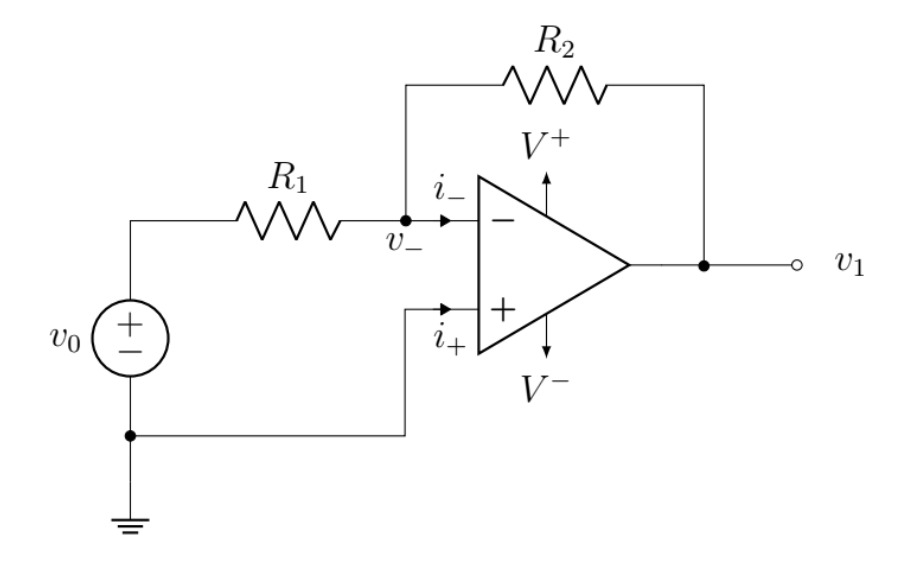
\includegraphics[scale=0.4]{figuras/circuito1}
\end{table}
\begin{center}
Figura 1: Disposição do Circuito 1
\end{center}

Esse circuito é um amplificador inversor, fazendo com que a tensão de saída seja inversa e de módulo maior que a tensão de entrada. 

Considerando um Amplificador Operacional ideal, devido ao conceito do curto virtual, $i_-=i_+=0$ assim como $v_-=v_+ =0$. Além disso, para um Amplificador Inversor, vale a relação $v_1=-\frac{R_2}{R_1}v_0$.

Os dados são coletados usando o Multímetro e seus resultados são dispostos na Tabela 2.

\vspace{5pt}
\begin{table}[h]
\centering
\begin{tabular}{|c|c|c|c|c|}
\hline
\textbf{Frequência (kHz)} & \textbf{Grandeza} & \textbf{Valor nominal} & \textbf{Valor medido} & \textbf{Erro (\%) }\\\hline
10   & $|V_0|$ & 1.57V & 1.55V & 1.27 \\\hline
10   & $|V_1|$ & 2.33V & 1.81V & 22.31 \\\hline
10   & $20log_{10}(|V_1|/|V_0|)$ & 3.434 & 1.347 & 60.77 \\\hline
10   & Fase de $V_1$ em relação a $V_0$ & -26.01\textdegree & -43.20\textdegree & 66.09 \\\hline
12.5 & $|V_0|$ & 1.25V & 1.38V & 10.40 \\\hline
12.5 & $|V_1|$ & 2.35V & 1.63V & 30.64 \\\hline
12.5 & $20log_{10}(|V_1|/|V_0|)$ & 5.481 & 1.446 & 73.62 \\\hline
12.5 & Fase de $V_1$ em relação a $V_0$ & -43.93\textdegree & -57.24\textdegree & 30.30 \\\hline
15.5 & $|V_0|$ & 0.97V & 1.34V & 38.14 \\\hline
15.5 & $|V_1|$ & 2.11V & 1.46V & 30.81 \\\hline
15.5 & $20log_{10}(|V_1|/|V_0|)$ & 6.733 & 0.745 & 88.94 \\\hline
15.5 & Fase de $V_1$ em relação a $V_0$ & -83.58\textdegree & -71.45\textdegree & 14.51 \\\hline
19.3 & $|V_0|$ & 1.17V & 1.34V & 14.53 \\\hline
19.3 & $|V_1|$ & 1.58V & 1.20V & 24.05 \\\hline
19.3 & $20log_{10}(|V_1|/|V_0|)$ & 2.626 & -0.958 & 136.48 \\\hline
19.3 & Fase de $V_1$ em relação a $V_0$ & -129.54\textdegree & -94.48\textdegree & 27.06 \\\hline
24.1 & $|V_0|$ & 1.51V & 1.47V & 2.65 \\\hline
24.1 & $|V_1|$ & 1.02V & 0.89V & 12.75 \\\hline
24.1 & $20log_{10}(|V_1|/|V_0|)$ & -3.381 & -4.359 & 28.93 \\\hline
24.1 & Fase de $V_1$ em relação a $V_0$ & -151.17\textdegree & -121.47\textdegree & 19.65 \\\hline
30   & $|V_0|$ & 1.72V & 1.64V & 4.65 \\\hline
30   & $|V_1|$ & 0.64V & 0.63V & 1.56 \\\hline
30   & $20log_{10}(|V_1|/|V_0|)$ & -8.635 & -4.155 & 51.88 \\\hline
30   & Fase de $V_1$ em relação a $V_0$ & -160.86\textdegree & -129.49\textdegree & 19.51 \\\hline
\end{tabular}
\caption*{Tabela 2: Valores referentes ao circuito 1}
\end{table}

Nota-se que por conta dos valores esperados serem 0, a fórmula de erro relativa não é muito adequada. No entanto, os valores medidos encontram-se dentro do esperado.

\newpage
Em seguida, é montado o circuito 2 que é um Amplificador não Inversor.

\begin{table}[h]
\centering
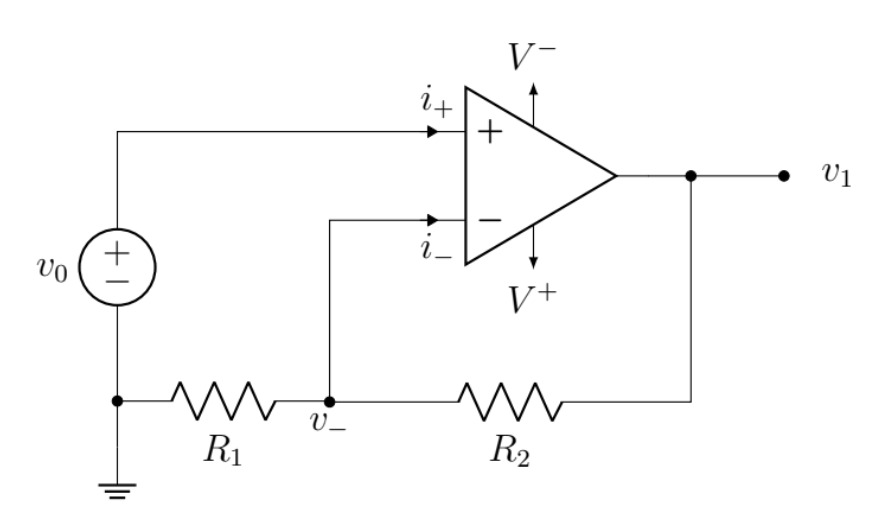
\includegraphics[scale=0.4]{figuras/circuito2}
\end{table}
\begin{center}
Figura 2: Disposição do Circuito 2
\end{center}

O procedimento é todo exatamente o mesmo, mudando apenas que para esse circuito o ganho é ditado por $v_1=(1+\frac{R_2}{R_1})v_0$.

Feitas todas as medições, os dados são dispostos na Tabela 3.

\vspace{5pt}
\begin{table}[h]
\centering
\begin{tabular}{|c|c|c|c|}
\hline
\textbf{Grandeza} & \textbf{Valor nominal} & \textbf{Valor medido} & \textbf{Erro (\%) }\\\hline
$v_0$ & 1V & 1.006V & 0.6 \\\hline
$v_1$ & 3.2V & 2.315V & 27.66 \\\hline
$v_-$ & 1V & 1.007V & 0.7 \\\hline
$V^+$ & 10V & 9.994V & 0.6 \\\hline
$V^-$ & -10V & -10.005V & 0.5 \\\hline
$i_+$ & 0A & 0.195A & - \\\hline
$i_-$ & 0A & 4.158mA & - \\\hline
\end{tabular}
\caption*{Tabela 1: Valores dos componentes}
\end{table}





\section{Conclusão}

\parag O estudo de Amplificadores Operacionais permitiu compreender suas principais características e comportamentos nas configurações utilizadas. Por meio de medições práticas, foi possível validar os conceitos teóricos relacionados ao amp-op, e destacou a versatilidade e a importância dos amplificadores operacionais no projeto de sistemas eletrônicos, reforçando seu papel fundamental em aplicações analógicas e digitais.

\section{Bibliografia}
\begin{itemize}
\item HALLIDAY, D.; RESNICK, R.; WALKER, J. Fundamentos de Física. 10. ed. v. 3. Rio de Janeiro: LTC, 2016.
\end{itemize}

\end{document}